%==============================================================================
% Sjabloon poster bachproef
%==============================================================================
% Gebaseerd op document class `a0poster' door Gerlinde Kettl en Matthias Weiser
% Aangepast voor gebruik aan HOGENT door Jens Buysse en Bert Van Vreckem

\documentclass[a0,portrait]{hogent-poster}

% Info over de opleiding
\course{Graduaatsproef}
\studyprogramme{Graduaat in het Programmeren}
\academicyear{2024-2025}
\institution{Hogeschool Gent, Valentin Vaerwyckweg 1, 9000 Gent}

% Info over de bachelorproef
\title{Unda Health Tracker}
\subtitle{Een Flutter Applicatie}
\author{Maïté De Smet}
\email{maite.desmet@student.hogent.be}
\supervisor{Luc Vervoort}
\cosupervisor{}

% Indien ingevuld, wordt deze informatie toegevoegd aan het einde van de
% abstract. Zet in commentaar als je dit niet wilt.
\specialisation{Programmeren}
\keywords{Health tracker, Flutter}
\projectrepo{https://github.com/MaitendoDS/graduaatsproef}

\begin{document}

\maketitle

\begin{abstract}
Voor mijn eindproject heb ik ervoor gekozen om een gezondheidstracker te maken in Flutter. Het is een mobiele app waar je een dagboek kan bijhouden van je symptomen, eetgewoonten en menstruatiecyclus.
\end{abstract}

\begin{multicols}{2} % This is how many columns your poster will be broken into, a portrait poster is generally split into 2 columns

\section{Introductie}
De Unda applicatie is een mobiele app ontwikkeld om gebruikers te helpen bij het tracken van hun gezondheid.
 Bij chronische gezondheidsproblemen wordt vaak aangeraden om verschillende soorten medische data bij te houden, 
 zoals een eetdagboek, menstruatiecyclus en pijnlogboek. 
 Het bijhouden van al deze gegevens in verschillende apps of notities kan verwarrend en inefficiënt zijn. 
 Daarom heb ik besloten om een centrale app te ontwikkelen waarin al deze functies worden samengebracht.

Met Unda heb je al je gezondheidsdata op één plek, waardoor je eenvoudig overzicht behoudt en deze informatie gemakkelijk 
met je arts kunt delen. Daarnaast maakt de app het mogelijk om patronen in je gezondheid te herkennen, wat kan bijdragen aan
 een betere behandeling of zelfinzicht.

Voor de ontwikkeling van deze app heb ik gekozen voor Flutter, een open-source UI-toolkit van Google voor het bouwen van 
applicaties voor iOS, Android, web en desktop vanuit één codebase. Flutter maakt gebruik van de programmeertaal Dart,
 een objectgeoriënteerde taal die eveneens door Google is ontwikkeld en geoptimaliseerd is voor UI-ontwikkeling.
\section{Wat heb ik bijgeleerd?}
Tijdens het ontwikkelen van de Unda app heb ik veel bijgeleerd over Flutter en Dart, zoals het gebruiken van widgets,
 dataopslag en app-navigatie. Ik leerde hoe je meerdere functies in één app integreert zonder het overzicht te verliezen.
Daarnaast verbeterde ik mijn probleemoplossend vermogen, leerde ik denken vanuit de gebruiker en werkte ik aan planning
 en doorzettingsvermogen. Dit project gaf me inzicht in zowel de technische als menselijke kant van app-ontwikkeling.

\section{Screenshot}

\begin{center}
  \captionsetup{type=figure}
  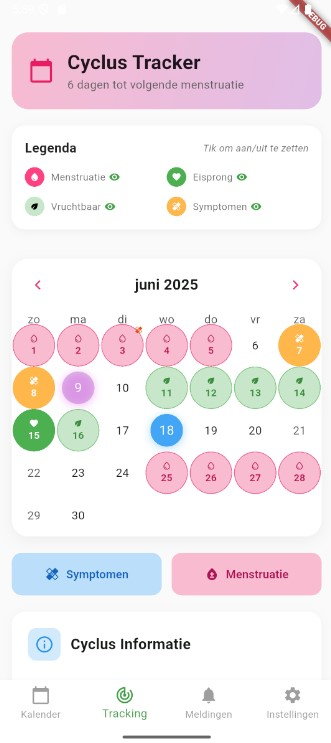
\includegraphics[width=0.5\linewidth]{hoofdscherm}
  \captionof{figure}{Dit is de hoofdpagina van de app}
\end{center}


\section{Conclusies}

Het ontwikkelen van de Unda app was een leerrijke ervaring waarin ik zowel mijn technische vaardigheden 
als mijn inzicht in gebruikersbehoeften heb versterkt. Ik ben trots op het resultaat en zie het als een 
waardevolle stap in mijn groei als ontwikkelaar.
\section{Toekomstig onderzoek}
Het gebruik van AI om patronen beter en sneller te herkennen. 
Meer functies, bijvoorbeeld het bijhouden van stoelgang en beweging. 
Koppeling met wearables.

\end{multicols}
\end{document}